\chapter{Introduzione: GeneroCity, un'Applicazione di SmartParking}

La crescente urbanizzazione e l'aumento del numero di veicoli in circolazione hanno reso la questione della mobilità urbana e della sosta un tema centrale per il futuro delle città. 
Le statistiche presentate dall'Osservatorio AIPARK\footnote{AIPARK - Associazione Italiana Operatori Sosta e Mobilità} nel giugno di quest'anno rivelano una situazione allarmante: l'Italia è al vertice della classifica europea per numero di autovetture, con un rapporto di 690 auto ogni 1.000 abitanti.Questa realtà comporta che circa il 30\% del traffico urbano sia generato da veicoli in cerca di parcheggio, evidenziando un disallineamento tra la domanda di sosta e l'offerta disponibile. Per correggere questo squilibrio è stato calcolato che sarebbe necessario aggiungere 670.000 posti auto, di cui oltre 200 mila solamente a Roma, dove, ad oggi, se ne conta uno ogni 39 residenti.\cite{ref:AIPARK}

Una possibile soluzione a questi problemi è lo \textbf{smart parking}, ossia una strategia che utilizza tecnologie digitali nel tentativo di utilizzare il minor numero di risorse possibili (carburante, tempo, spazio) per ottenere un processo di sosta dei veicoli più veloce, facile e ottimizzato.\cite{ref:smartparking}

\begin{figure}[h]
    \centering
    
\includegraphics[width=0.5\linewidth]{images/gc_logo.png}
    \caption{Logo di GeneroCity}
    \label{fig:gc_logo}
\end{figure}
\section{GeneroCity e il suo scopo}
In questa realtà nasce GeneroCity: un’applicazione di smart parking in sviluppo per Android e iOS realizzata dal Gamification Lab del Dipartimento di Informatica della Sapienza Università di Roma. Lo scopo dell'applicazione è quello di facilitare lo scambio dei parcheggi all’interno di un’area urbana puntando sulla generosità degli utenti\cite{ref:generocity}: la sua idea principale è quella di rilevare quando un utente esce da un parcheggio e segnalarlo agli utenti che ne stanno cercando uno nella stessa zona. Inoltre sono presenti i \textit{GCoins}, ossia una moneta virtuale che gli utenti guadagnano cedendo il loro posto ad altri e possono spendere per prenotarne uno. 
\begin{wrapfigure}{r}{0.5\textwidth}
    \centering
    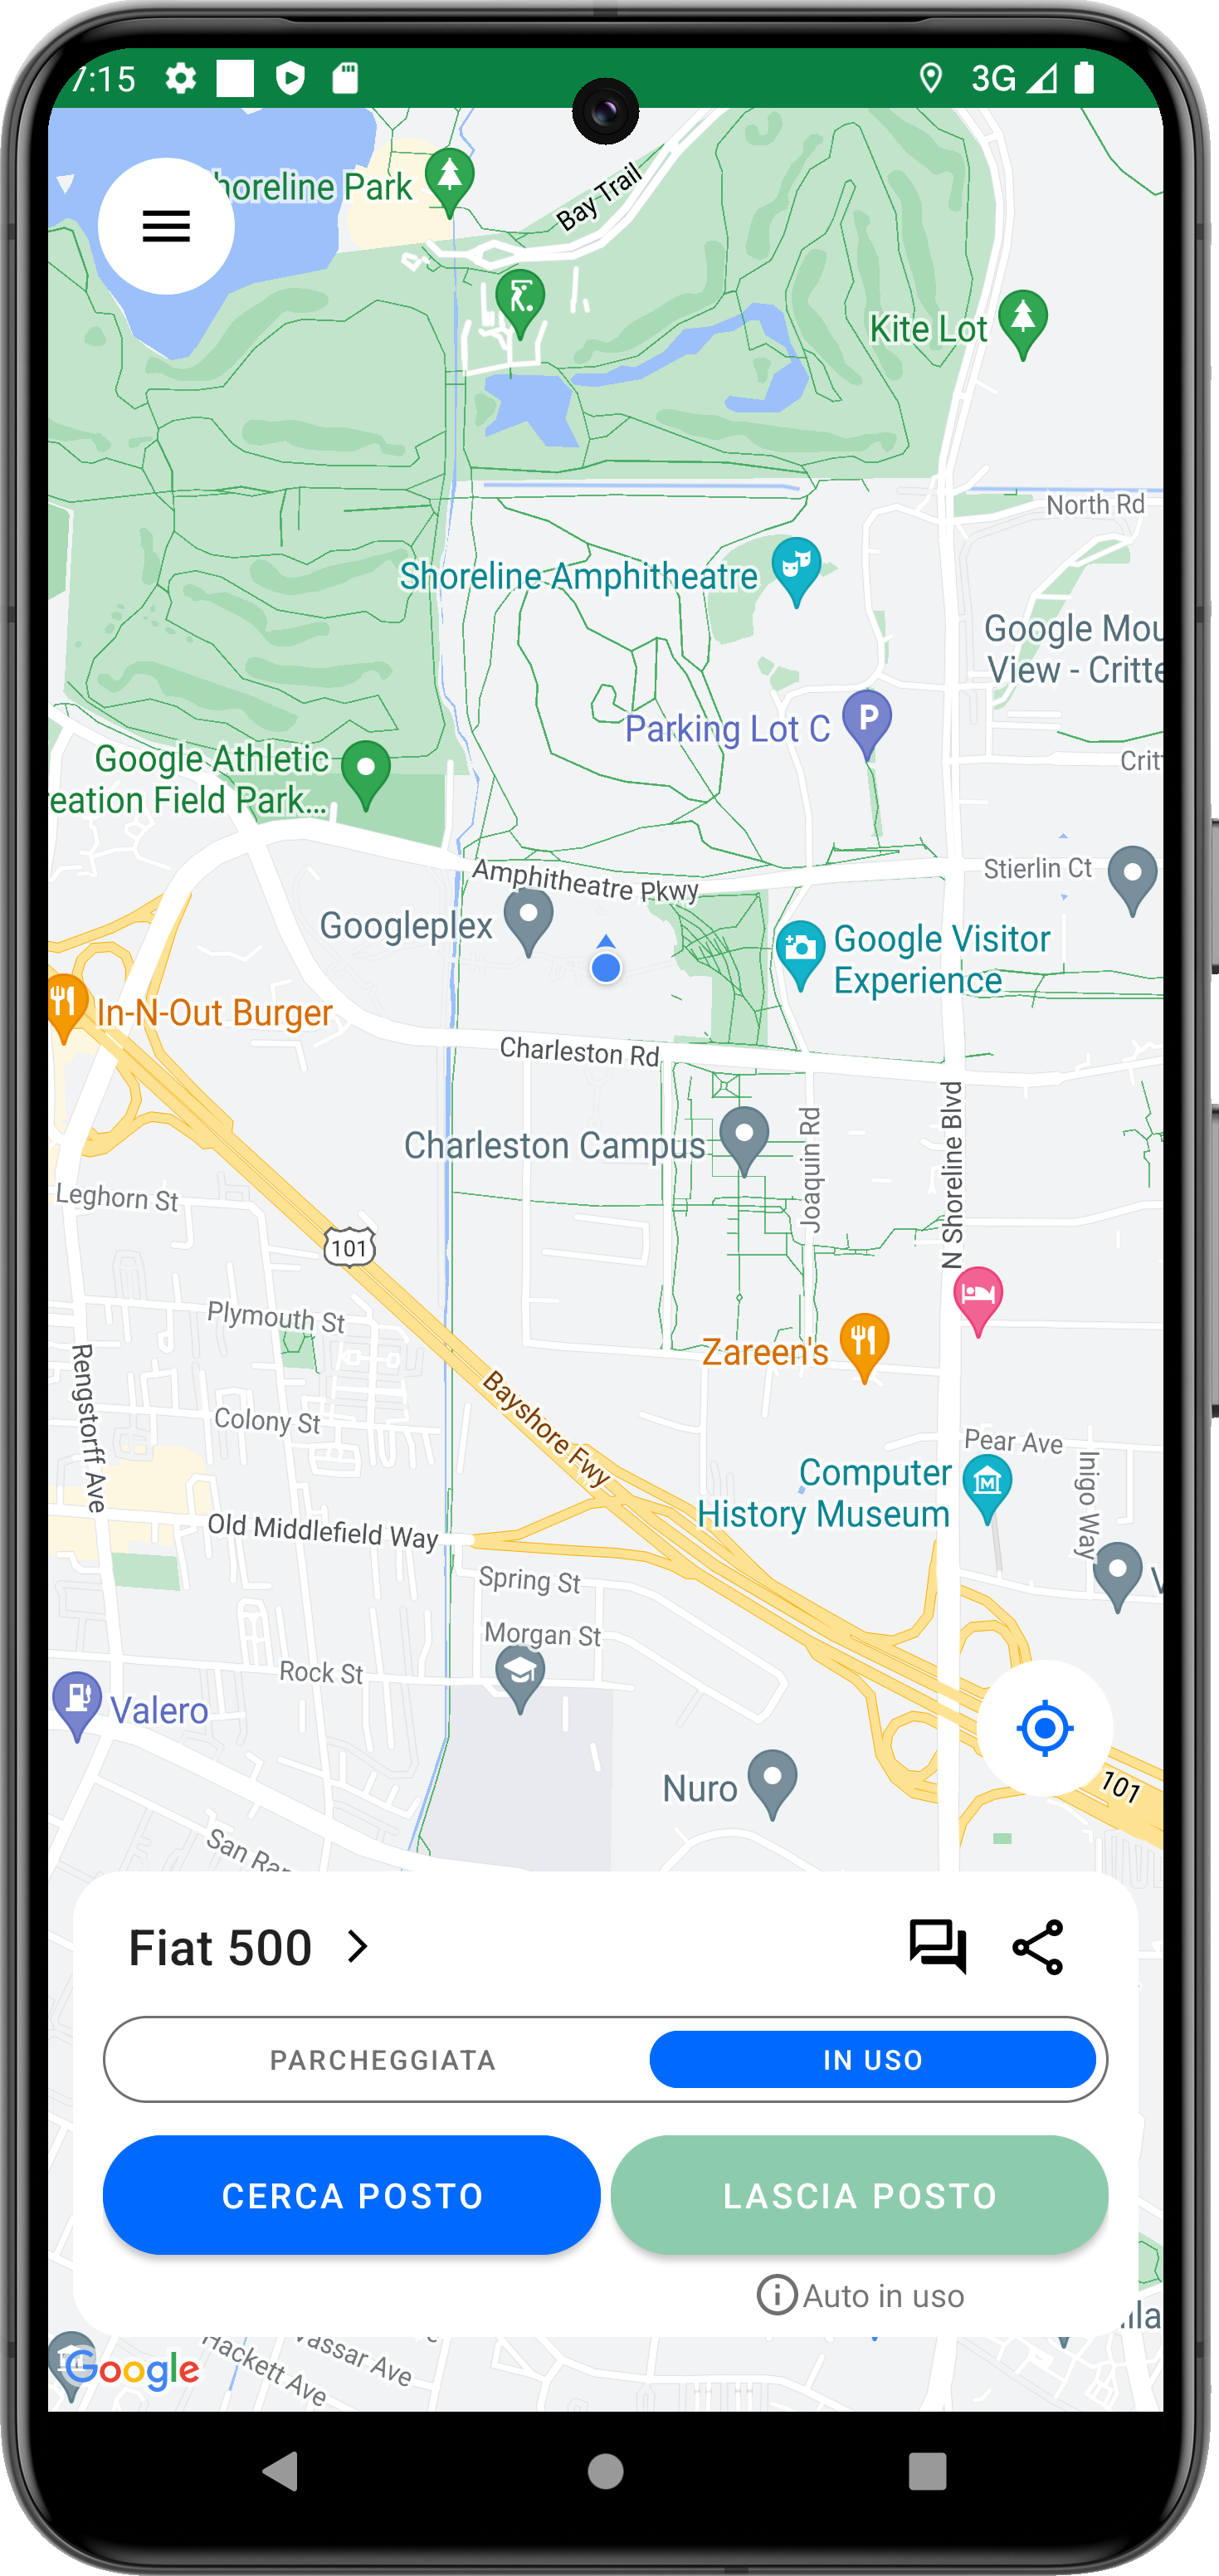
\includegraphics[width=0.9\linewidth]{images/gc_main_activity.png}
    \caption{GeneroCity Android}
    \label{fig:main_screen}
\end{wrapfigure}
Essi rappresentano una componente di gamification\footnote{La gamification è l'utilizzo di elementi mutuati dai giochi e delle tecniche di creazione di giochi in contesti non ludici.} con lo scopo di motivare e coinvolgere gli utenti ad utilizzare l'applicazione.

La vera innovazione introdotta da questo progetto però, è il numero limitato di interazioni che l'utente dovrà avere con essa: l'applicazione cercherà di prevedere automaticamente quando quest'ultimo lascia o cerca un parcheggio, ciò in modo da garantire una maggiore sicurezza alla guida. Il mio ruolo nello sviluppo di GeneroCity è stato quello di utilizzare le funzionalità bluetooth degli smartphone Android per raggiungere tale scopo.
